\chapter{Object level vision}
\minitoc

We will develop two measurements models that have in common to relate a camera pose to a known object in the environment through a rigid transformation. The first one 
is derived from Apriltag fiducial markers \cite{wang2016iros}, which are widely used in the robotics community. The second uses a deep learning-based method
to obtain relative poses from objects whose CAD models are known \cite{labbe2020cosypose}. Our main contribution is to develop covariance models for both
models so as to be able to use them in the context of multi-sensor fusion.

We assume that the camera has been calibrated and that the images are corrected against distortions. The camera reference frame
follows the convention X-Y-Z = Righ-Down-Front.

\section{General factor}
Let's assume that an algorithm provides us $\Tm{C}{O} \in \SE(3)$, a measurement of the pose of an element 
of the scene with an attached frame $O$ with respect to the camera frame $C$ located at the Camera optical frame.
The kinematic chain of the problem described in \figRef{fig:camera_object_chain} unrolls as 
$\T{W}{O} = \T{W}{B}\T{B}{C}\T{C}{O}$ where W and B correspond to the world and body frames.
Given measurement $\Tm{C}{O}$, this relation can therefore be turned into a residual relating 
the robot pose, the camera extrinsics, and the object pose:

\begin{equation}
    \bfr (\T{W}{B}, \T{B}{C}, \T{W}{O}) = \Log(\T{W}{O} \T{W}{B}^{-1} \T{B}{C}^{-1} \T{C}{O}^{-1}) ~ \in \Reals^6
\end{equation}

We also assume that we have access to the covariance of this measurement 
\mbox{$\Cov_V \in \Reals^{6 \times 6}$}. We will now describe two applications of this factor, one using Apriltag fiducial markers and one using 
a deep-learning object pose estimation algorithm.

\begin{figure}
    \centering
    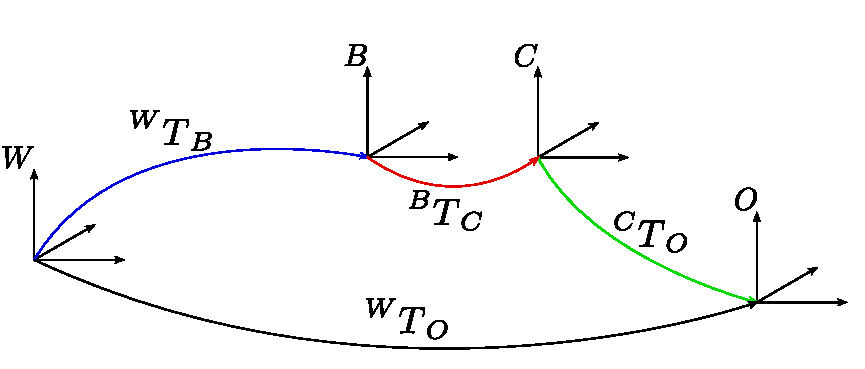
\includegraphics[width=0.7\textwidth]{figures/kin_tree_object.pdf}
    \caption{Kinematic tree of the object/camera measurement model}
    \label{fig:camera_object_chain}
\end{figure}


%
%
\section{Fiducial marker}
\subsection{Markers Pose estimation algorithms}

Fiducial markers are widely used in robotics and Augmented Reality (AR) applications as they provide an easy way to obtain a relative 6D pose 
between a calibrated camera and the marker. These markers are designed so that they are easily uniquely and robustly identifiable in any scene 
\cite{wang2016iros,romero2018speeded}. For square markers, the outputs of the algorithm are sub-pixel projections of the square corners, whose 
corresponding position in the local reference frame of the tag is known (using the tag dimensions). Recovering their pose is then an example 
of the Perspective n Point (PnP) algorithm, which requires at least three 2D-3D correspondences to compute the 3D pose. 
A vast literature has been written on the topic, many of them relying on efficient analytical models
\cite{gao2003complete, lepetit2009epnp, collins2014infinitesimal, terzakis2020consistently}, sometimes refined by a nonlinear maximum likelihood step. 

A known problem of fiducial markers is the orientation ambiguity for noisy images. Close to fronto-parallel pose (identical orientation as 
the camera frame, null x and y position), the estimated orientation can jump from orientations several tenths of degrees apart \cite{collins2014infinitesimal}. 
This problem has been addressed by an analytical algorithm called Infinitesimal Plane-based Pose Estimation \cite{collins2014infinitesimal} that can 
provide both ambiguous solutions so that the end-user may make an informed choice based on other data.

\subsection{Covariance model}
Obtaining a covariance of the estimated transformation is an important step toward the integration of these measurements in a sensor fusion algorithm.
For methods relying on a maximum likelihood nonlinear refinement step, one might invert the Hessian matrix at the optimum to obtain a covariance.
Others \cite{urban2016mlpnp} rely on maximum likelihood estimation and a careful parameterization of the homogeneous coordinates associated to
2D features. Eq. (23) \cite{urban2016mlpnp} shows an analytical formula to compute pose uncertainty from pixel noise. However the formulation is 
particular to the choice of parameterization described in the paper and, therefore, we think that a simpler formulation is possible. This model is proposed 
in our work \cite{fourmy2019absolute}. 

Usually, when a nonlinear mapping of noise variables from one space to another is available, we can linearize the model with respect to the noise
to obtain a first-order approximation of the propagated uncertainty (\cite{barfoot2017state} Eq. 7.337).  
Instead of directly obtaining Jacobians from the PnP algorithms, we found that a natural way to proceed is to take the opposite 
direction. It should somehow be possible, knowing the marker size and the relative pose measurement, and assuming pixel noise, to
recover $\Cov_{O}$. A simple model of this noise is to assume isotropic Gaussian noise on the pixels. If we stack four pixel (the four tag corners) 
$\bfx_i = [u_i, v_i] \in \Reals^2$ and we stack then in the vector $\bfx = [\bfx_1 \bfx_2 \bfx_3 \bfx_4]$, we have therefore that
$\bfx$ is corrupted by a Gaussian noise $\Cov_{\bfx} = \sigma_{x}^2 \bfI_8$, where $\sigma_{x}$ usually takes values of 1 or 2 pixels.
PnP algorithm provides us with a function $\text{pnp}$ defined as:

\begin{equation}
    \begin{split}
        f: \Reals^8 &\rightarrow \SE(3) \\
                           \bfx &\rightarrow \T{C}{O} = \text{pnp}_w(\bfx)
    \end{split}
\end{equation}

where w denotes the dependency on the width of the marker. This $\text{pnp}_w$ function implementation depends on the specificities of the PnP algorithm used and  
is in general hard to analytically differentiate. Instead, if we consider the inverse function

\begin{equation}
    \begin{split}
        g: \SE(3) &\rightarrow \Reals^8 \\
                           \T{C}{O} &\rightarrow \bfx = \text{proj}_w(\T{C}{O})
    \end{split}
\end{equation}

that maps the relative pose to the projection of the tag in the image, a rather simple jacobian expression can be derived using the chain rule, as follows.

Let's define the marker corner coordinates in the marker frame, like shown in \figRef{fig:tag_coordinate_frame}. As a convention 
\cite{wang2016iros} we order the corners counter-clockwise starting from bottom left (looking straight at the tag). 

\begin{equation}
    c =
    \begin{pmatrix}
    c_1 \\ c_2 \\ c_3 \\ c_4
    \end{pmatrix}
    ~~
    c_1 =  \begin{pmatrix} -\frac{w}{2} \\ \frac{w}{2} \\ 0 \end{pmatrix}
    ~ 
    c_2 =  \begin{pmatrix} \frac{w}{2} \\ \frac{w}{2} \\ 0 \end{pmatrix}
    ~
    c_3 =  \begin{pmatrix} \frac{w}{2} \\ -\frac{w}{2} \\ 0 \end{pmatrix}
    ~
    c_4 =  \begin{pmatrix} -\frac{w}{2} \\ -\frac{w}{2} \\ 0 \end{pmatrix}
\end{equation}.

%
\begin{figure}
    \centering
    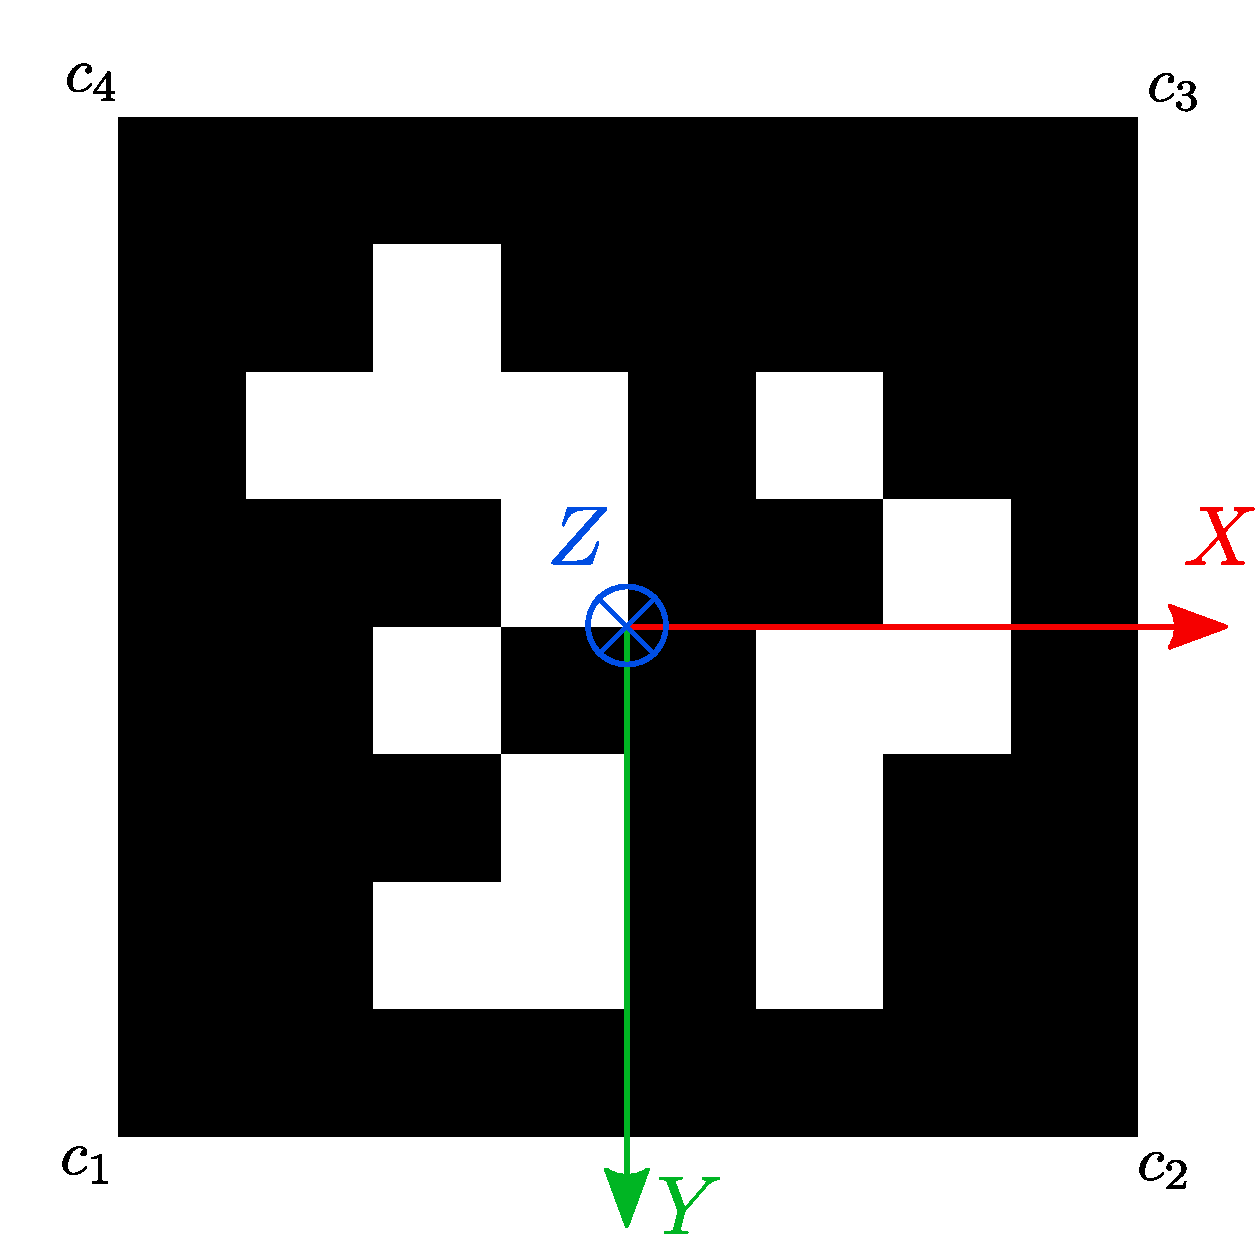
\includegraphics[width=0.5\textwidth]{figures/tag12_frame.pdf}
    \caption{Apriltag local coordinate systems and corners conventions \cite{wang2016iros}}
    \label{fig:tag_coordinate_frame}
\end{figure}

Then, assuming that images are corrected (no distortion), the pinpoint camera model gives us that

\begin{equation}
    \bfx_i = \text{eucl}(h_i) = \text{eucl}(K\T{C}{O} c_i)
\end{equation}
for each corner $c_i$, where $h_i$ are the homogeneous coordinates representing the projected corners and $eucl$ is the euclideanization function defined as
\begin{equation}
    \begin{split}
        \text{eucl}: \Reals^3 &\rightarrow \Reals^2 \\
        \bfh = \begin{pmatrix}x\\y\\z\end{pmatrix} &\rightarrow \bfx = \begin{pmatrix}x/z\\y/z\end{pmatrix}
    \end{split}
\end{equation}

We need to compute the jacobian of each corner projection with respect to the estimated relative pose $J^{x_i}_{\T{}{}} = J^{x_i}_{h_i} J^{h_i}_{\T{}{}}$. 
Regarding the transformation, we will consider it to be an element of $\Reals(3)\times \SO(3)$ since the translation and rotation part 
of transformation are treated separately in our solver. The expressions of those functions are therefore expressed as:

% DROP dependency on C L for clearer notation?
\begin{equation}
    \begin{split}
        &h_i = K(\Rot{C}{O}c_i + \posi{C}{O}) \\
        &J^{h_i}_{\posi{C}{O}} = K ~~~~~~ J^{h_i}_{\Rot{C}{O}} = -K\Rot{C}{O}[c_i]_{\times}  \\  
        &J^{h_i}_{\T{C}{O}} = [J^{h_i}_{\posi{C}{O}} ~J^{h_i}_{\Rot{C}{O}}] = K [I_3 ~~~ -\Rot{C}{O} [c_i]_{\times}]
    \end{split}
\end{equation}
while the euclideanization jacobian is found to be
\begin{equation}
    J^{x_i}_{h_i}
    =
    \begin{pmatrix}
    1/z_i & 0 & -x_i/z_i^2 \\
    0 & 1/z_i & -y_i/z_i^2
    \end{pmatrix}
\end{equation}


Finally, we can stack the 4 jacobians to get the full jacobian to be used for covariance propagation.
\begin{equation}
    J \triangleq J^{\bfx}_{\T{C}{O}}=
    \begin{pmatrix}
    J^{\bfx_1}_{\T{C}{O}} \\ J^{\bfx_2}_{\T{C}{O}} \\ J^{\bfx_3}_{\T{C}{O}} \\ J^{\bfx_4}_{\T{C}{O}}
    \end{pmatrix}
    ~ \in \Reals^{8 \times 6}
\end{equation}.


We therefore have the covariance propagation equation $\Cov_{\bfx} = J \Cov_{\T{C}{O}} J^T$. 
This equation must be inverted in order to recover the needed covariance. $J$ being non square, 
we have to use the pseudo inverse to write: $\Cov_{\T{C}{O}} = J^{T,\dagger} \Cov_{\bfx} J^{\dagger}$. 
Given that the pixel noise covariance is isotropic as explained above, this equation simplifies to:

\begin{equation}
\Cov_{\T{C}{O}} = \sigma_{\bfx}^2(J^T J)^{-1}    
\end{equation}

Note that the derivations above are not limited to a square tag with four corners and could in theory be used for any object defined as
a set of points in its local coordinate system, provided their configuration is not degenerate and makes the PnP computation possible \cite{gao2003complete}.  
We have therefore a compact model informed by the geometry of the measurement model with  a single tuning parameter in the pixel noise $\sigma_\bfx$.

It is hard to represent graphically the appearance of this uncertainty model from the full 6D covariance. However, we can inspect the positional and orientational
(respectively 3x3 upper-left and 3x3 lower-right sub-matrices) by representing theme as confidence ellipsoids.
In fact, for a random variable $x$ with a size $k$ multivariate normal distributions with mean $\mu \in \Reals^3$ and 
covariance matrix $\Cov \in \Reals^{3 \times 3}$, the statistics:
%
\begin{equation}
    (x - \mu)^T \Cov^{-1}(x - \mu) = \chi^2
    \label{eq:chi2}
\end{equation}
%
follows a chi-square distribution with 3 degrees of freedom. We can then plot confidence volumes as ellipsoids by replacing the right end side of  
\eqRef{eq:chi2} by the critical value of the chi-square distribution for the desired confidence interval (we chose $\alpha=99\%$). We simulate a 
realistic scenario using calibration data from a laboratory Realsense camera, 15cm tags a $\sigma_\bfx = 2$. An example of a simulated scene is given
in \figRef{fig:apriltag_cov}. 

\begin{figure}[h]
    \centering
    \begin{subfigure}{.49\linewidth}
        \centering
        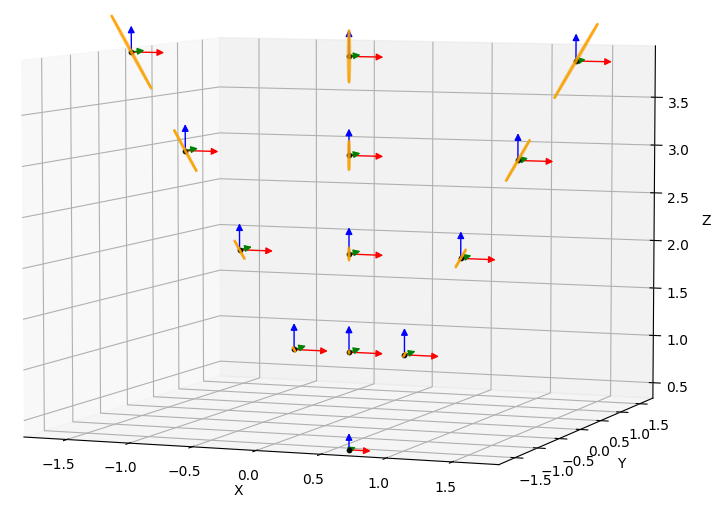
\includegraphics[width=\textwidth]{figures/apriltag_cov_posi.png}
        \caption{Relative position covariances \label{fig:apriltag_cov_posi}}
    \end{subfigure}%
    \hfill
    \begin{subfigure}{.49\linewidth}
        \centering
        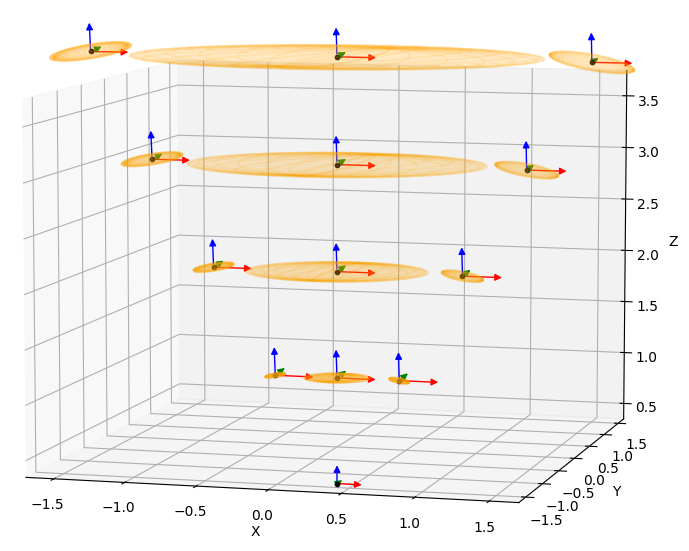
\includegraphics[width=\textwidth]{figures/apriltag_cov_orientation.png}
        \caption{Relative orientations covariances \label{fig:apriltag_cov_orientation}}
    \end{subfigure}%
    \caption{Representation of the analytic covariance model. The single frame at the bottom represents the pose of the virtual camera, others are identical 
    apriltags placed in front of the camera at different distances but identical orientations, covariances are represented in orange, centered at the corresponding taf position.
    (\subref{fig:apriltag_cov_posi}) shows that the main positional uncertainty is along the camera-tag axis, which corresponds to the depth information. 
    (\subref{fig:apriltag_cov_orientation}) shows that in contrary the rotation along the camera-tag axis is by far the most precise.}
    \label{fig:apriltag_cov}
\end{figure}

We can see that the error distribution is clearly anisotropic. The uncertainty of the pose measurements
is logically higher in the dimensions that lead the least change in the aspect of the tag projection. For a fronto-parallel tag, the highest 
uncertainty is along the z-axis, which corresponds to a high depth uncertainty.
In \figRef{fig:apriltag_proj}, 3 tags are projected: the first (black) is half a meter away from the camera in fronto-parallel orientation, the second (orange)
to the right and the third (rose), 10cm behind. We can see that the appearance of difference of appearance due to a depth-wise movement is much smaller, which 
explains the higher uncertainty on the depth measurement. A similar observation can be made for orientation as well. 

\begin{figure}[h]
    \centering
    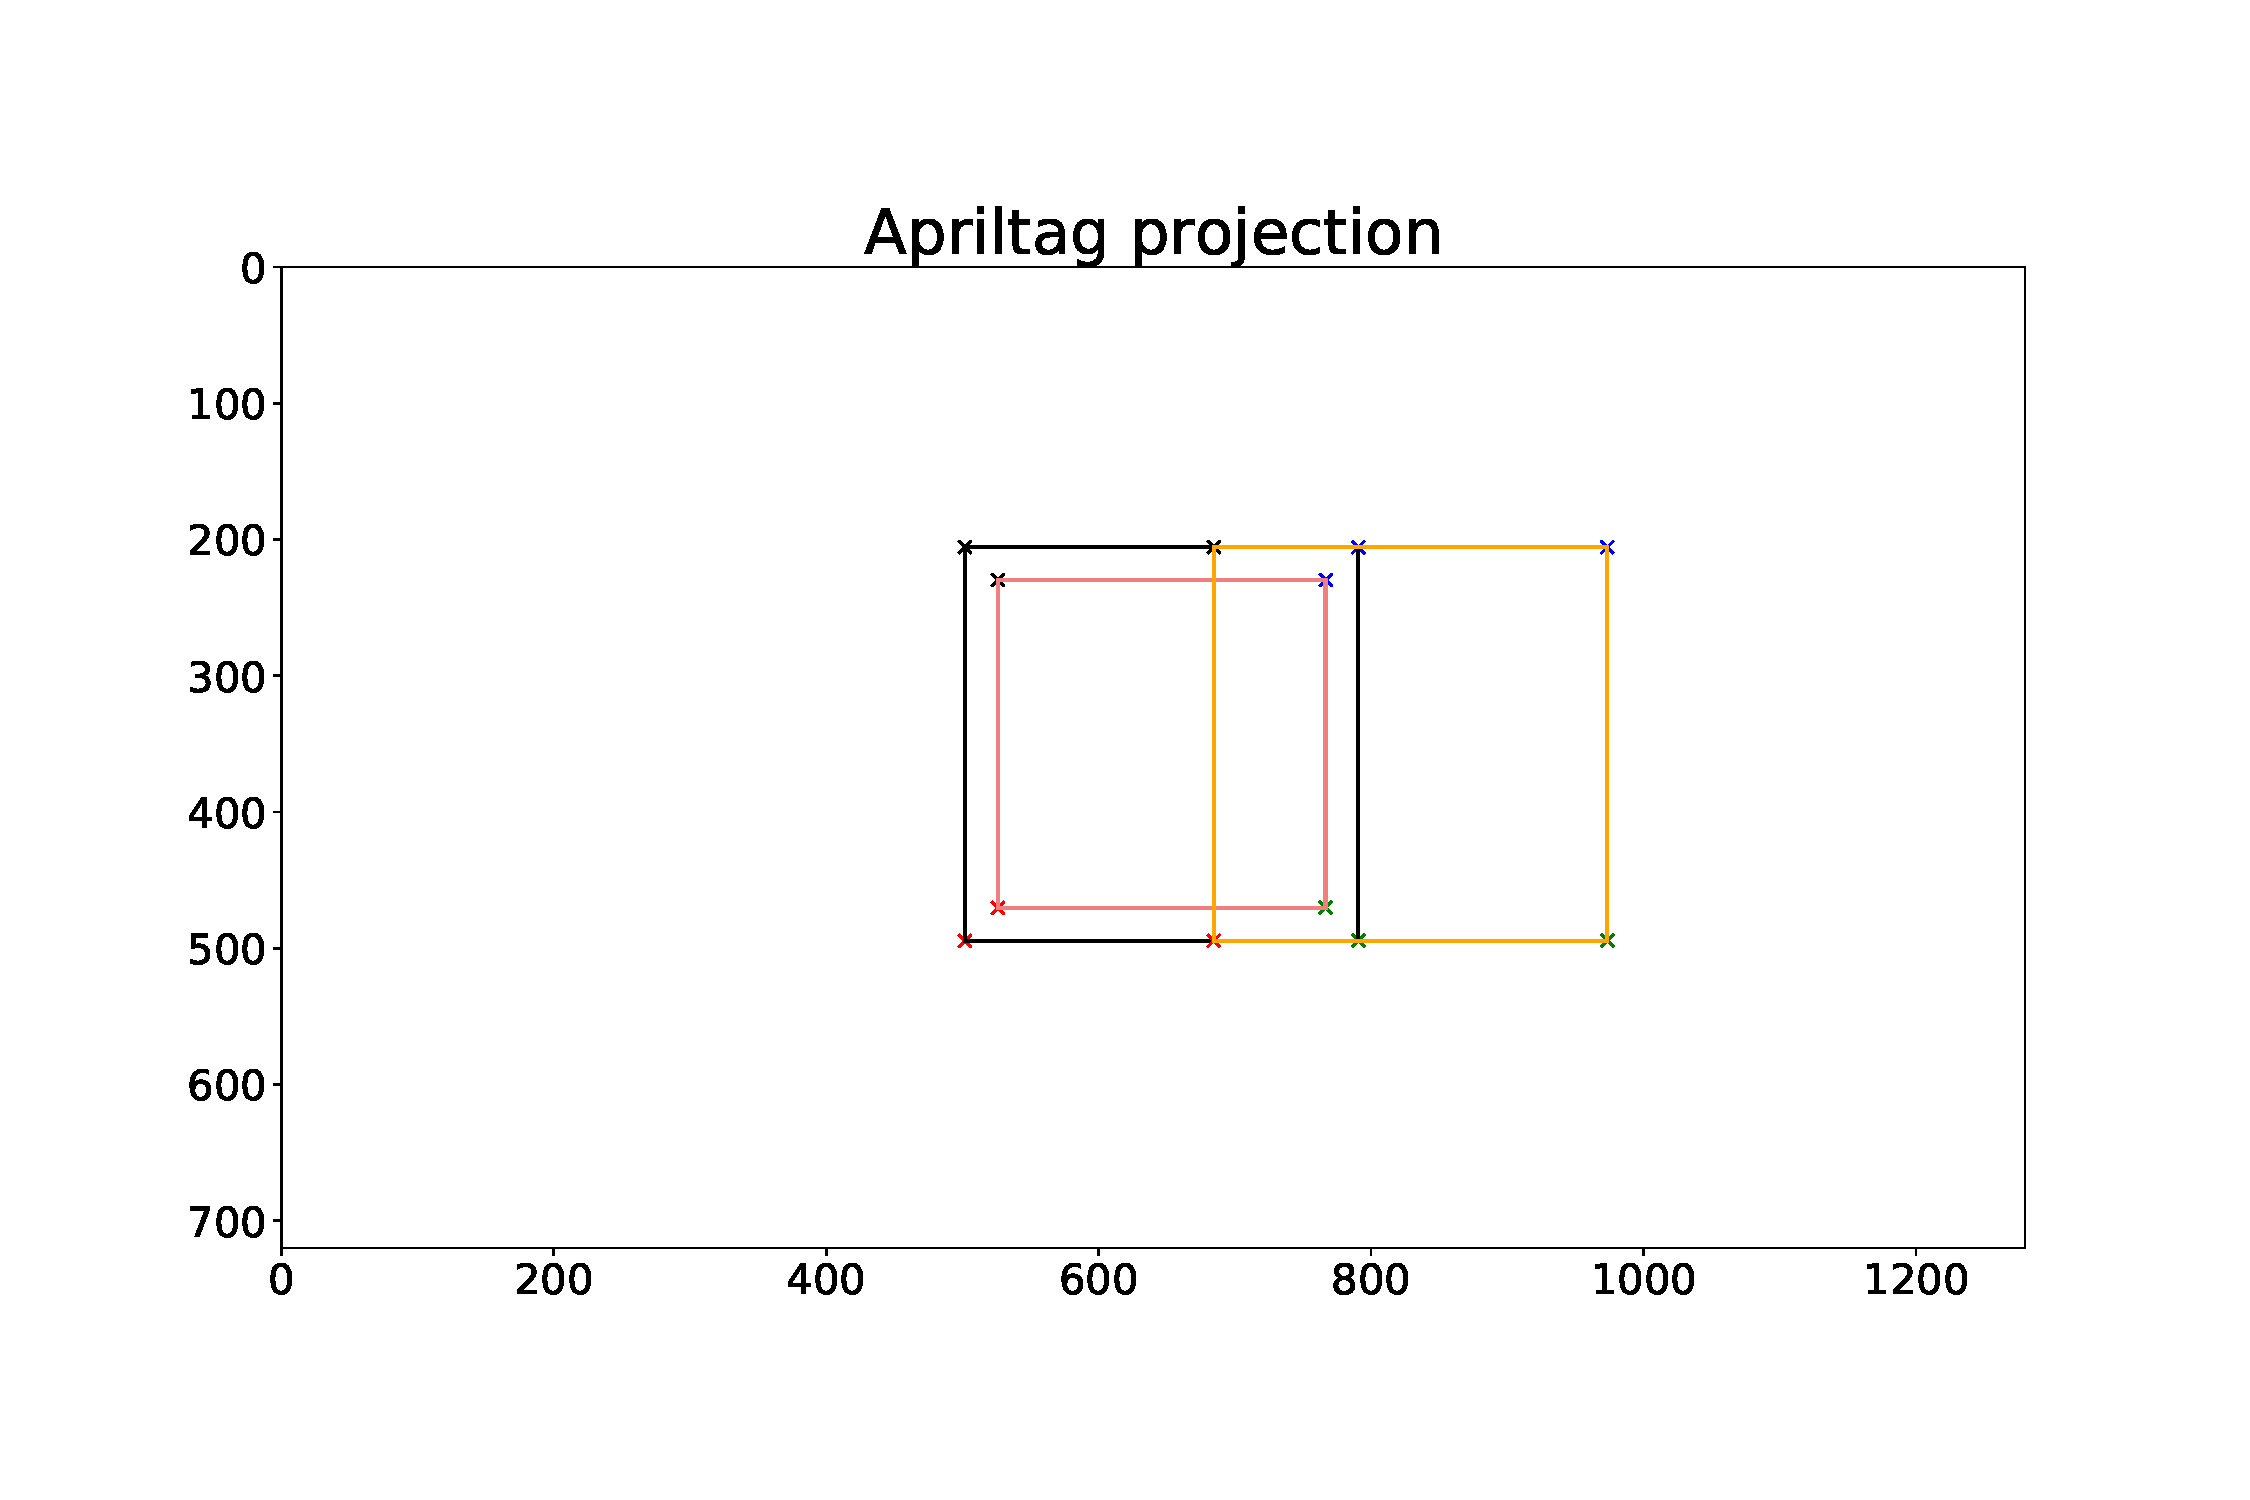
\includegraphics[width=0.8\textwidth]{figures/apriltag_proj.pdf}
    \label{fig:apriltag_proj}
    \caption{Projection of 3 tags of camera frame position: black -> (0,0,0.5), orange -> (0.1,0,0.5), rose -> (0.0,0,0.6)}
\end{figure}

A quantitative comparison with \cite{urban2016mlpnp} would be interesting as well as an experimental validation campaign.


\subsection{Ambiguity in the pose estimation}
It is well known that the pose extraction from planar markers suffers from an inherent ambiguity between two fairly different rotations as described in 
\cite{8206468} for instance. One solution is to define the tag factor residual as the pixel error between the detected corners and their projection given 
current tag pose estimate and let the optimizer find the most probable tag poses given the complete set of measurements. However if one tag is wrongly initialized, 
the optimizer is not guaranteed to leave the local minimum with new measurements. Our solution is to bring the disambiguation on the front-end side.
\cite{collins2014infinitesimal} provides an implementation of the PnP problem that retrieves both ambiguous poses. When expressed in camera frame, 
both solutions share the tag position and differ only in its orientation. We typically want to select the solution with smaller error. 
However, if the reprojection errors $e_1$ and $e_2$ are too close (we test for $\tfrac{e_2}{e_1} < h$ with $e_1 \leq e_2$ and $h$ an empirical threshold), 
we increase the rotational part of the covariance matrix by a great factor to prevent a potential wrong tag orientation to influence the estimation.


%
\section{Learning-based object pose estimation}
In this section, we propose to integrate a deep-learning-based object pose estimation algorithm \cite{labbe2020cosypose} to our measurement models. 


\subsection{Object pose estimation algorithms}
The problem of object pose estimation can simply be stated: given a calibrated camera and a set of known object models, detect those objects in the current image 
frame and extract camera-objects poses. Traditionally, competing methods were developed using either local features matching or learning-based methods.
As shown by the most recent BOP challenge results [cite], deep-learning methods now clearly dominate the field in terms of accuracy. 
At the time of the writing, the highest-ranking non-learning-based pose extraction method \cite{konig2020hybrid} (object detection is deep learning-based) 
actually uses depth measurement measurements and is dominated by a purely RGB, deep-learning-based models \cite{haugaard2021surfemb}, though it seems to be ten 
times faster \footnote{BOP challenge leaderboard is available at \url{https://bop.felk.cvut.cz/leaderboards/}}.

These results advocate for the use of purely RGB image-based results, which now provide accurate enough results for these to be used in robotics applications 
\cite{labbe2021single}. We use the work of Labbe et al. \cite{labbe2020cosypose} which at the time ranked first in the BOP challenge leaderboard.
This approach mixes a new state-of-the-art single-view pose estimation algorithm with a multi-view algorithm using RANSAC and Bundle Adjustment. 
It achieved first in most of the 2020 BOP challenge categories \cite{hodavn2020bop}. This system obtains precision in the order of centimeters 
on real objects whose 3D model is known. Its performances make it a good candidate as a direct 6D pose sensor to perform multi-sensor fusion. 
In the context of legged robots, this is very useful to localize the robot with respect to objects it needs to interact with, such as objects 
to manipulate or stairs to climb. While these models are not yet able to be generalized to classes of objects, rapid progress is expected in 
this direction. Their performances are already very interesting to help with the locomotion in known scenes.

\subsection{CosyPose}
The front end of the SLAM system designed for this project includes object detection and object pose estimation. 
This function is provided by CosyPose \cite{labbe2020cosypose}, a deep learning-based 6D tracker that reaches state-of-the-art
 performances for 6D object pose estimation. % and which was awarded at the BOP contest \cite{hodan2020bop}. 
In the original paper, a single-view pose estimator and a multi-view algorithm were introduced. In our context, only the single-view module is used, 
while object tracking is handled by the SLAM framework. 

CosyPose takes as input a single image $I$ and a set of 3D models, each associated with an object label $l$. The camera $C$ is assumed to be calibrated. 
A set of object detections is performed using the object detector Mask-RCNN \cite{he2018mask}. Then, each 2D candidate detection in view $I$ is identified 
by an index $\alpha$ and associated with an object candidate $O_{\alpha}$ and its 6D pose $\T{C}{O_{\alpha}} \in \SE (3)$ with respect to the camera $C$.

\begin{figure}[]

    \begin{subfigure}{.5\textwidth} % this sets the figure to be max half the width of the page
        \centering
        % include first image
        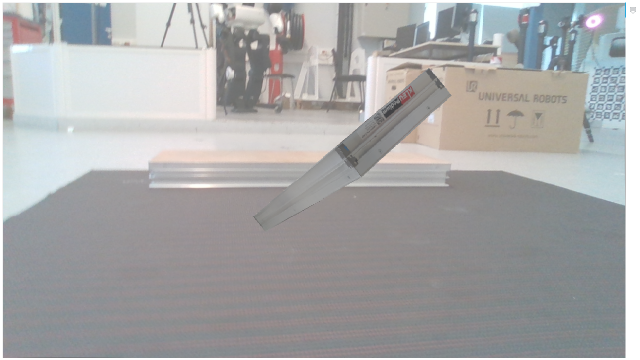
\includegraphics[width=.9\linewidth]{figures/convergence_1.png}  % this sets the image to fill 90% of the available space -> 45% of the line width in total. 
        % \caption{\label{fig:cosypose-convergence_1}}
    \end{subfigure}
    \begin{subfigure}{.5\textwidth}
        \centering
        % include second image
        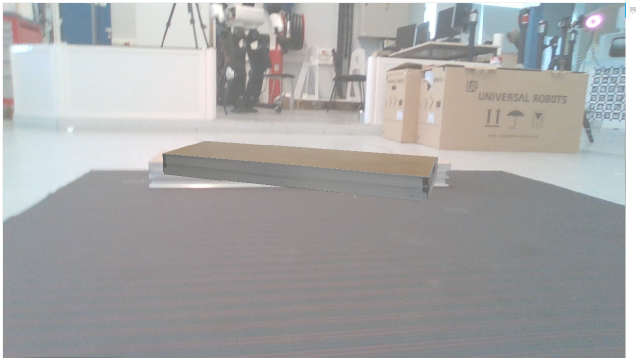
\includegraphics[width=.9\linewidth]{figures/convergence_2.png}  
        % \caption{\label{fig:cosypose-convergence_2}}
    \end{subfigure}

    \label{fig:fig}
    \begin{subfigure}{\textwidth}
        \centering
        % include first image
        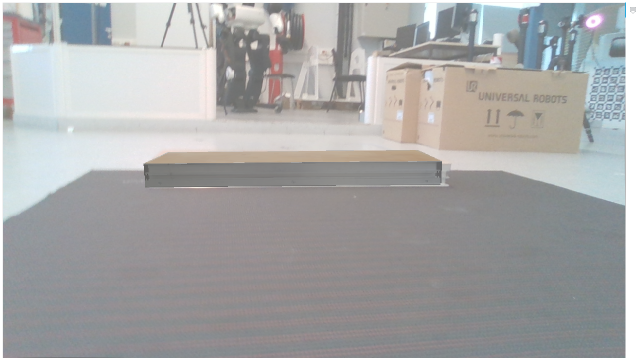
\includegraphics[width=.45\linewidth]{figures/convergence_3.png}   % this width should be half of the width of the other two images
        % \caption{\label{fig:cosypose-convergence_3}}
        
    \end{subfigure}
    \caption{\label{fig:cosypose-convergence} Progressive convergence of a stair step estimated pose over successive iterations of CosyPose.}
\end{figure}


The single-view pose estimation procedure of CosyPose is an improvement over the one proposed in DeepIm \cite{deepim_2019}. The general idea is to iteratively 
use the same neural network to converge to the most precise object pose (\figRef{fig:cosypose-convergence}). It takes as input the cropped image of the bounding 
box of the detected object and a rendered image-based on the current object pose solution $\T{C}{O_{\alpha},k-1}$ at iteration $k-1$. 
It returns a transformation update $\T{O_{\alpha},k-1}{O_{\alpha},k}$ that brings the rendered image closer to the cropped image. In practice, 
two neural networks with the same structure are trained independently: one for coarse pose estimation, \ie, the first iteration of the iterative process, 
and one for the refinement of the pose, \ie, the last iterations. The coarse network gives the first transformation $\T{C}{O_{\alpha},0}$, 
and the prediction of the pose of the object is obtained by composing the $N$ successive transformations:

\begin{equation}
\T{C}{O_{\alpha}} = \T{C}{O_{\alpha},0} \prod_{k=1}^N  \T{O_{\alpha},k-1}{O_{\alpha},k}
\end{equation}

CosyPose reuses the neural network architecture of DeepIm with a new backbone for feature extraction: Efficient-Net \cite{tan2020efficientnet} 
with a spatial average pooling layer added after it. Then, it disables the optical flow sub network during the training. 
A new rotation parametrization is used for the loss function which was introduced in \cite{zhou2020continuity} and which has been shown 
to bring more stability during training. Then, the focal length of the cropped images is recomputed during training to fit the virtual camera 
of these images. Finally, the object symmetries are taken into account during training thanks to the \textit{symmetric distance}. 
Each 3D model $l$ is associated with a set of symmetries $S(l)$, that is the set of transformations that leave the aspect of the object unchanged:

\begin{equation}
    \textit{S}(l) = \left \{ \bfS \in \SE(3) | \forall \bfT \in \SE(3), \mathcal{R}(l,\bfT) = \mathcal{R}(l,\bfT \bfS)\right \}
\end{equation}

where $\mathcal{R}(l,\bfT)$ is the rendered image of the object $l$ captured in pose $M$. Given a set of symmetries $S(l)$, 
we define the symmetric distance $D_l$ which measures the distance between two 6D poses represented by transformation $\bfT_1$ and $\bfT_2$. 
Given an object $l$ associated to a set $\mathcal{X}_l$ of 3D points $\mathbf{x} \in \mathcal{X}_l$, we have:

\begin{equation}
    D_l(\bfT_1, \bfT_2) = \underset{\bfS \in \textit{S}(l)}{\text{min}} \frac{1}{|\mathcal{X}_l|} \sum_{\mathbf{x} \in \mathcal{X}_l} ||\bfT_1 S\mathbf{x} - \bfT_2\mathbf{x} ||^2
    \label{eq:distSym}
\end{equation}

Equation (\eqRef{eq:distSym}) measures the average distance between the points of the object model transformed by $\bfT_1$ and $\bfT_2$ according to the symmetry 
that best aligns the transformed points. In practice, for continuous symmetries  that are rotations around an axis (like for instance for a textureless cylinder), 
$S(l)$ is discretized using 64 angles.


\subsection{Empirical covariance estimation}

When considering merging a tracker such as CosyPose with other sensor modalities, an important aspect is to predict covariance representing the level 
of confidence in the tracker estimate. Such data uncertainty is crucial to the robustness of SLAM systems involving neural networks 
subsystems such as \cite{yang2020d3vo}, while \cite{SalasMoreno2013SLAMSL} claimed to compute a covariance matrix approximated as the inverse of the 
Iterative Closest Point output. The methods targeted for deep learning applications are harder to implement, especially if the goal 
is to use an off-the-shelf pose estimation neural network, as it is the case for this paper. For instance, Bayesian Neural Networks \cite{jospin2020hands} 
need to be trained explicitly for uncertainty prediction while Monte Carlo (MC) Dropout \cite{gal2016dropout} requires multiple forward passes at run-time.

In our work CosySLAM \cite{debeunne2021cosyslam}, we present a practical implementation of a SLAM system based on the design of an off-the-shelf deep learning object 
pose estimation algorithm \cite{labbe2020cosypose}, which empirical results are presented in section [REF]. 
In order to be able to integrate these measurements with other sensors, we propose a noise model based on empirical data.

\subsubsection{Covariance model}

CosyPose does not provide an evaluation of its uncertainty.
%
The two main families of solutions available to estimate uncertainties of neural network predictions consist in MC dropout \cite{gal2016dropout} 
or Bayesian Neural Network (BNN) \cite{jospin2020hands}. Using BNNs would require to change the architecture of CosyPose and to retrain it. 
MC dropout would require several forward passes through the network for each iterations, which would be computationally expensive. 

We need to compute the covariance without changing the architecture of the network and at an affordable cost. 
We propose to make an empirical error model based on polynomial regression in order to compute the covariance matrix. 
The idea is to parametrize the average error on each $\se(3)$ component returned by CosyPose. We conduct an empirical study on several video 
sequences that explore the variations of the parameter set for several object types. The error is computed by comparing the $\SE(3)$ transformations 
between the camera $C$ and an object $O$ returned by CosyPose $\T{C}{O}$ with the same transformation given by a motion capture system. 
We then use the error predictions of our parametric model as a proxy to the true 6 covariances during model fitting. 
A different model is fit for each object type due to their diversity of shapes, sizes and textures.

The parameters to compute the error need to represent as much as possible the error sources of CosyPose. 
To cover the error due to the configuration of the object in space, we need to include the 3D coordinates of the camera in the object frame. 
We also want to take into account some invariance that can occur by rotating around the object if it is texture-less for example. 
For this reason, we choose spherical coordinates of the camera origin with respect to the object frame to parametrize the model. 
Another source of error can be the occlusion of the object in the scene, as well as the motion blur, or any inherent noise in the image. 
This can affect the quality of the detection and of the pose estimation. Having an idea of the quality of the object detection informs us on the 
quality of the object representation that may be occluded or blurry. The Mask-RCNN object detector returns a confidence score $s$ for each detection 
that we will include in our model. This score is the output of the final softmax layer of the detector, which is designed to represent a probability distribution.

% To sum up, we have the following parameters for our error model:
% \begin{itemize}
% \item $\displaystyle r = || \posihat{O}{C}||$,
% \item $\displaystyle \varphi  = \arctan\left(\frac{ \prescript{0}{}{\hat{x}}_C}{\prescript{0}{}{\hat{y}}_C}\right)$,
% \item $\displaystyle \theta  = \arcsin\left(\frac{\prescript{0}{}{\hat{z}}_C}{r}\right)$,
% \item $\displaystyle s$ : mask-RCNN softmax output.
% \end{itemize}

To sum up, our model is parametrized by four values: $r$ - distance, $\varphi$ - azimuth, $\theta$ - elevation, $s$ - Mask-RCNN softmax output. 
We can then compute the error of CosyPose with respect to the motion capture data: 

\begin{equation}
    \mathbf{e}  = [\mathbf{e}_{t}, \mathbf{e}_{a}]  \triangleq  \left[~\posihat{O}{C} - \posim{O}{C}, ~ \Log \left(\Rothat{O}{C}^{-1}\Rotm{O}{C}\right)~\right]
\end{equation}

where $\widehat{\cdot}$ and $\widetilde{\cdot}$ denote quantities obtained from the motion capture system and CosyPose respectively. 
$\Log$ denotes the logarithm application mapping elements of SO(3) to the $\Reals^3$ representation of its Lie algebra 
$\so(3)$.

We want to find a polynomial function $f(r, \varphi, \theta, s) \in \mathbb{R}^6$ that returns the error given the set of training data $\{X,E\}$. 
For each object, we capture a set of video sequences and we compute the error with the motion capture data for each measurement. 
We then perform polynomial regression with a pipeline in Scikit Learn \cite{scikit-learn}. A simple linear regression leads to a high root-mean-square error (RMSE) 
on a test dataset. Over degree 3, the model overfits and the high curvature of the polynomial returned high error values outside of the training data range. 
Thus, a degree 2 polynomial regression seemed to offer a good compromise.  Quantitative results are given in the experimental validation section 
(see Fig.~\ref{fig:empirical_err} for a few examples of fitted polynomials).


\subsubsection{Empirical covariance}

As explained in Sec. II, we have trained empirical models to evaluate the covariance of the estimation of CosyPose. 
To validate these models, we propose to exhibit a few intuitive observations and a quantitative statistical analysis. 
One of the parameter involved in our model is the absolute distance between the camera and the object, noted $r$. 
Our trained models show an expected behavior regarding this parameter: the global error increases when the camera moves away from the object. 
%
\begin{figure}[h]
  \centering 
  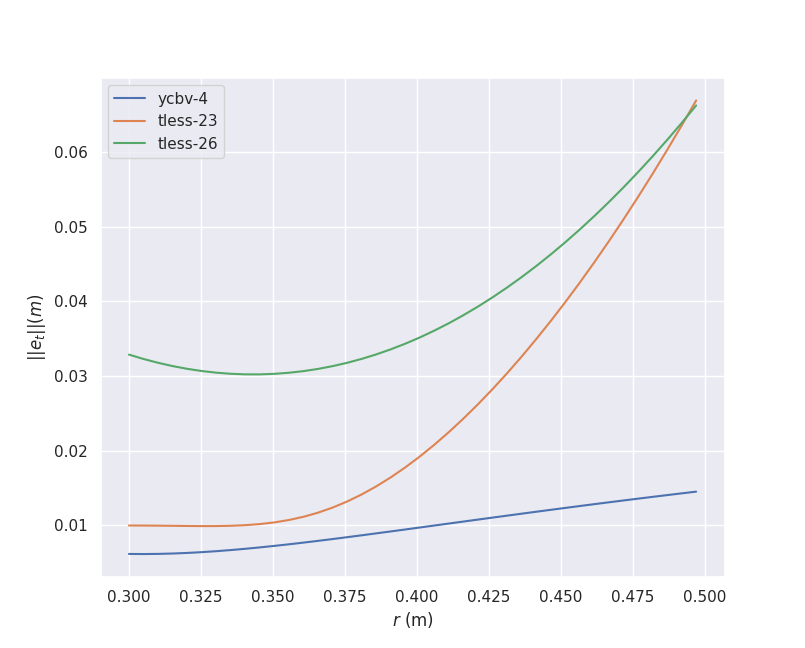
\includegraphics[width=0.8\textwidth]{figures/empirical_err.png}
  \caption{The norm of the translation error returned by the models of three different objects with respect to $r$, the distance between the camera and the object. 
            The other parameters $\theta$, $\phi$ and $s$ are fixed to the average values of our training data. }
  \label{fig:empirical_err}
\end{figure}

\figRef{fig:empirical_err} sheds light on these phenomena and gives an explicit comparison between the models of different objects. 
The error of the object from the YCBV dataset seems more stable and smaller than the one of the objects from the T-LESS dataset. 
This can be explained by the texture of the object and the absence of symmetries: T-LESS objects are known to be more challenging 
for pose estimation and this is confirmed by our model.

A more quantitative evaluation can be deduced from table \tabRef{table:empirical_models}. The translation error seems to be captured pretty well,
 as the RMSE is around the centimeter. However, the angular error seems a little less predictable, especially for T-LESS objects which orientation 
 estimation can suffer from an important measurement noise due to the lack of textures. The $R^2\in[0,1]$ score is the coefficient of determination 
 and is often used to evaluate statistical models. Its interpretation is subject to debate and cannot conclude to a "good" or a "bad" model. 
 However, a score higher than 0 demonstrates that our model is more accurate than a simple average model.

\begin{table}[h]
    \centering
    \begin{tabular}{|c|c|c|c|}
        \hline 
          & $\displaystyle R^{2}$ & RMSE ang. err. (°) & RMSE trans. err. (cm) \\
        \hline 
         YCBV-4 & 0.55 & 5,1 & 0.6 \\
        \hline 
         T-LESS-23 & 0.5 & 11.7 & 1.5 \\
        \hline 
         T-LESS-26 & 0.68 & 22 & 0.6 \\
         \hline
    \end{tabular}
    \caption{A quantitative evaluation of our models, these values are computed on test samples that were not used for training. }
    \label{table:empirical_models}
\end{table}
